\chapter{Vector Geometry}

Vectors provide valuable assistance when it comes to describing geometric objects. In this chapter, we are going to exploit the knowledge learnt in the previous chapters to solve geometry problems and inspect more deeply the intimate relationship between vectors, \textit{dot/cross products}, and geometry.

\section{Lines and Planes}
\textit{(Straight) lines} and \textit{planes} are geometric shapes of importance in two/three-dimensional real spaces ($\mathbb{R}^2$ and $\mathbb{R}^3$) and due to their simplicity they will be frequently seen. They can be expressed either in terms of (a) an equation, and (b) vectors. We will start from the easier case of a line. Since a straight line is a one-dimensional object, the vector form of such a line can be expressed by a fixed vector that points to its initial position, plus another vector oriented along the line's direction, times an arbitrary parameter that controls its extension or contraction, so that it traces out the line when the parameter changed continuously.
\begin{figure}[ht!]
    \centering
    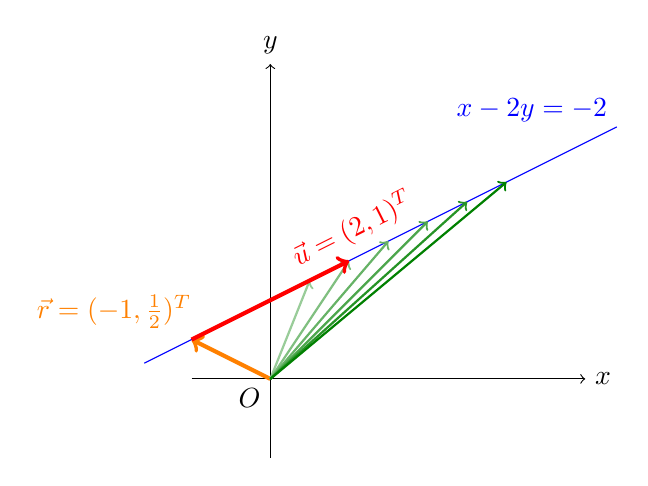
\begin{tikzpicture}
\draw[->] (-1,0)--(4,0) node[right]{$x$};
\draw[->] (0,-1)--(0,4) node[above]{$y$};
\draw[line width=1.5, orange, ->] (0,0)--(-1,0.5) node[above left, xshift=4]{$\vec{r} = (-1,\frac{1}{2})^T$};
\draw[blue] (-1.6, 0.2)--(4.4, 3.2) node[left, yshift=6]{$x - 2y = -2$};
\draw[Green!40, thick, ->] (0,0)--(0.5,1.25);
\draw[Green!50, thick, ->] (0,0)--(1,1.5);
\draw[Green!60, thick, ->] (0,0)--(1.5,1.75);
\draw[Green!70, thick, ->] (0,0)--(2,2);
\draw[Green!85, thick, ->] (0,0)--(2.5,2.25);
\draw[Green, thick, ->] (0,0)--(3,2.5);
\draw[line width=1.5, red, ->] (-1,0.5)--(1,1.5) node[above, pos=1.1, sloped]{$\vec{u} = (2,1)^T$};
\node[below left]{$O$}; 
\end{tikzpicture}
    \caption{\textit{The graph of $\color{blue}x - 2y = -2$ can take the vector form of $\smash{\color{Green}\overrightarrow{OP}} = {\color{orange}\vec{r}} + {\color{Green}t} {\color{red}\vec{u}} = {\color{orange}(-1,\frac{1}{2})^T} + {\color{Green}t}{\color{red}(2,1)^T}$. The orange/red arrow represents the initial position/direction, and the locus of the green arrow is controlled by $\color{Green}t$ like a slider. The cases for $\color{Green}t = 0.75, 1, 1.25, 1.5, 1.75, 2$ are shown.}}
    \label{fig:vectraceline}
\end{figure}\par
Short Exercise: Choose any value of $t$ for the example in Figure \ref{fig:vectraceline} and substitute that value into the expression of $\smash{\overrightarrow{OP}}$ above to see if the $x$ and $y$ components satisfy the starting equation. Also, try to increase/decrease the value of $t$ to observe how the vector traces out the desired straight line.\footnote{Let's say $t = -0.25$, $\overrightarrow{OP}=(-1,0.5)^T + (-0.25)(2,1)^T = (-1.5, 0.25)^T$, $x - 2y = (-1.5) - 2(0.25) = -2$.}

\subsection{Translating Equation Form to Vector Form}
The general equation form of a line on an $xy$ plane is $ax + by = h$, resembling a linear system of one equation with two unknowns. From Section \ref{subsection:SolLinSysGauss}, it can be observed that it has infinitely many solutions and possesses a free variable. Let $y = t$, then rearranging the equation we have $x = (h - bt)/a$ where $t$ is any scalar. Denote the origin as $O$ and any point on the line as $P$, then 
\begin{align*}
\overrightarrow{OP} =
\begin{bmatrix}
x \\
y
\end{bmatrix}
=
\begin{bmatrix}
\frac{h}{a} - \frac{b}{a}t\\
t
\end{bmatrix}
= 
\begin{bmatrix}
\frac{h}{a}\\
0
\end{bmatrix}
+ t
\begin{bmatrix}
-\frac{b}{a}\\
1
\end{bmatrix}
\end{align*}
This is one possible vector form (\textit{parameterization}) of the line. Its idea can be borrowed from Example \ref{exmp:mulsol}, with $\smash{(\frac{h}{a}, 0)^T}$ being the initial position/particular solution, and $\smash{(-\frac{b}{a}, 1)^T}$ as the direction of that line, multiplied by a free parameter (complementary solution) to complete the general solution. For example, if we have $3x - 2y = 5$, then by the same method, we get
\begin{align*}
\begin{bmatrix}
x \\
y
\end{bmatrix}
=
\begin{bmatrix}
\frac{5}{3} + \frac{2}{3}t\\
t
\end{bmatrix}
= 
\begin{bmatrix}
\frac{5}{3}\\
0
\end{bmatrix}
+ t
\begin{bmatrix}
\frac{2}{3}\\
1
\end{bmatrix}    
\end{align*}
Bear in mind that the direction vector (representing complementary solution) can be scaled freely. In addition, any initial position vector (particular solution) can be chosen as long as it connects to a point on the line and satisfies the equation. (You may refer to the discussion about particular/complementary solutions in Section \ref{subsection:SolLinSysGauss}.) Hence, there is no unique vector form for a line. For instance,
\begin{align*}
\begin{bmatrix}
1\\
3
\end{bmatrix}
+ t_1
\begin{bmatrix}
2 \\
4
\end{bmatrix}     
\end{align*}
is equivalent to
\begin{align*}
\begin{bmatrix}
-1\\
-1
\end{bmatrix}
+ t_2
\begin{bmatrix}
1 \\
2
\end{bmatrix}     
\end{align*}
for the line equation $2x - y = -1$.\par
Short Exercise: Check the equivalence of the two vector forms above by choosing a value for $t_1$ and finding the corresponding $t_2$ so that the vector points to the same position.\footnote{For example, if $t_1 = 1$, we have $(1, 3)^T + (1)(2, 4)^T = (3,7)^T$ as a point on the line, and for the other vector form $(-1,-1)^T + t_2(1, 2)^T = (3,7)^T$ to coincide we will have $t_2 = 4$. In this case, it can be shown that the general relation between the two forms is determined by $t_2 = 2t_1 + 2$, as
\begin{align*}
\begin{bmatrix}
1\\
3
\end{bmatrix}
+ t_1
\begin{bmatrix}
2 \\
4
\end{bmatrix}
=
\left(
\begin{bmatrix}
-1\\
-1
\end{bmatrix}
+
\begin{bmatrix}
2 \\
4
\end{bmatrix}
\right)
+ 2t_1
\begin{bmatrix}
1 \\
2
\end{bmatrix}
=
\begin{bmatrix}
-1\\
-1
\end{bmatrix}
+ (2t_1+2)
\begin{bmatrix}
1 \\
2
\end{bmatrix}
\end{align*}}\\
Short Exercise: What is the vector form of the equation $ax + by = h$ for the degenerate case $a=0$?\footnote{The equation is reduced to $y = \frac{h}{b}$ and we select $x = t$ as the free variable instead.\\ 
$\begin{bmatrix}
x \\
y
\end{bmatrix}
=
\begin{bmatrix}
t \\
\frac{h}{b}
\end{bmatrix}
=
\begin{bmatrix}
0 \\
\frac{h}{b}
\end{bmatrix}
+
t
\begin{bmatrix}
1 \\
0
\end{bmatrix}$}

\subsection{Recovering Equation Form from Vector Form} On the other hand, inferring a line equation from the vector form is not straightforward at first sight. Since the vector form of a line always contains an arbitrary parameter, which is absent in the equation form, the motivation is to remove the parameter through some manipulation. Remember that from Properties \ref{proper:dotorth} the dot product between orthogonal (perpendicular) vectors returns zero. This means that by carrying out a dot product with the \index{Normal Vector}\keywordhl{normal vector} of the line, which is orthogonal to the direction vector, on both sides of the vector form, we will eliminate the parameter and recover the line equation. For example, given that
\begin{align*}
\begin{bmatrix}
x\\
y
\end{bmatrix}
=
\begin{bmatrix}
1\\
3
\end{bmatrix}
+ t
\begin{bmatrix}
1 \\
4
\end{bmatrix} 
\end{align*}
We know that $(4, -1)^T$ is a normal vector orthogonal to the direction vector (see the next short exercise). So, by taking dot product with $(4, -1)^T$ on both sides, we have
\begin{align*}
\begin{bmatrix}
x\\
y
\end{bmatrix}
\cdot
\begin{bmatrix}
4\\
-1
\end{bmatrix}
&=
\left(\begin{bmatrix}
1\\
3
\end{bmatrix}
+ t
\begin{bmatrix}
1 \\
4
\end{bmatrix}\right)
\cdot
\begin{bmatrix}
4\\
-1
\end{bmatrix}
=
\begin{bmatrix}
1\\
3
\end{bmatrix}
\cdot
\begin{bmatrix}
4\\
-1
\end{bmatrix}
+ t
\begin{bmatrix}
1 \\
4
\end{bmatrix} 
\cdot
\begin{bmatrix}
4\\
-1
\end{bmatrix}\\
4x - y &= ((1)(4) + (3)(-1)) + ((1)(4)+(4)(-1))t = 1 + 0t = 1 \\
\Rightarrow 4x - y &= 1
\end{align*}
Notice that the coefficients of the equation are the same as the components of the normal vector. \par
Short Exercise: Verify that $(a, b)$ is always normal/orthogonal to $(b, -a)$, and vice versa.\footnote{$(a, b)^T \cdot (b, -a)^T = (a)(b) + (b)(-a) = 0$}

\subsection{Generalizing to Higher Dimensions}
\label{section:vecgeohighdim}
Similar concepts can be applied on the equation and vector form for planes. General form of the equation of a plane in three-dimensional space is $ax + by + cz = h$, which is a linear system of one equation with three unknowns. From the analysis in Section \ref{subsection:SolLinSysGauss} we know there are two free variables and two (non-parallel) direction vectors for such a plane. By assigning any two (non-pivotal) unknowns as the free variables, we then obtain the vector form of the plane. 
\par
Recall from Section \ref{section:crossprod}, that the cross product of any two non-parallel vectors on the plane will give a third vector normal to the plane. Subsequently, we can take the dot product with this newly obtained normal vector to convert the vector form back to a plane equation just like what we have done for a line in the last subsection. Again, the coefficients of the plane equation match the components of the normal vector, differing at most by a multiplicative factor.
\begin{figure}[ht!]
    \centering
    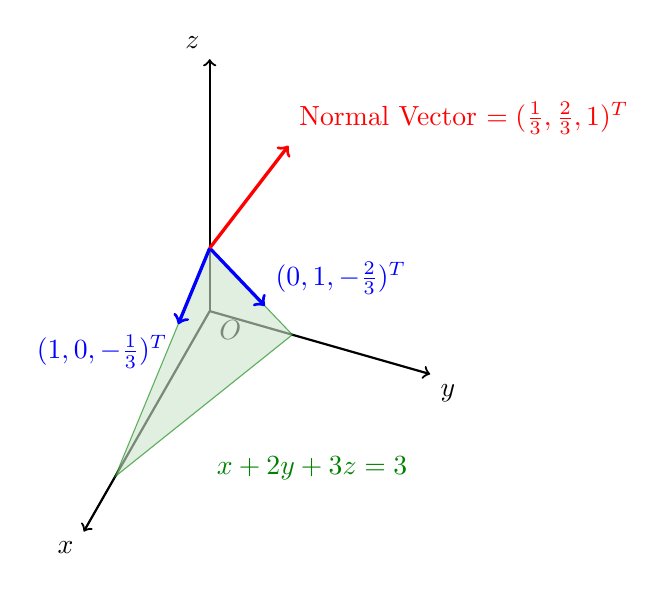
\begin{tikzpicture}[x={(-0.4cm, -0.7cm)}, y={(0.7cm, -0.2cm)}, z={(0cm, 0.8cm)}]
\node[below right]{$O$}; 
\draw[thick,->] (0,0,0) -- (4,0,0) node[anchor=north east]{$x$};
\draw[thick,->] (0,0,0) -- (0,4,0) node[anchor=north west]{$y$};
\draw[thick,->] (0,0,0) -- (0,0,4) node[anchor=south east]{$z$};
\filldraw[draw=Green, fill=Green!20, opacity=0.6]
(3,0,0) -- (0,3/2,0) -- (0,0,1) -- cycle;
\node[Green] at (2,3) {$x + 2y + 3z = 3$};
\draw[very thick,->,blue] (0,0,1) -- (1,0,2/3) node[below left]{$(1, 0, -\frac{1}{3})^T$};
\draw[very thick,->,blue] (0,0,1) -- (0,1,1/3) node[above right]{$(0, 1, -\frac{2}{3})^T$};
\draw[very thick,->,red] (0,0,1) -- (1,2,4) node[above right]{Normal Vector $= (\frac{1}{3}, \frac{2}{3}, 1)^T$};
\end{tikzpicture} 
    \caption{\textit{The plane represented by the equation $x + 2y + 3z = 3$. Notice that the normal vector can be found via computing $\smash{(1, 0, -\frac{1}{3})^T} \times \smash{(0, 1, -\frac{2}{3})^T} = \smash{(\frac{1}{3}, \frac{2}{3}, 1)^T}$. The normal vector is magnified for the purpose of illustration.}}
\end{figure}

\begin{exmp}
\label{exmp:vecgeohighdim}
Transform the plane equation $2x+3y+z = 4$ to vector form and convert the acquired vector form back to the starting equation to verify consistency.
\end{exmp}
\begin{solution}
For the first part, we can let $y=s$, $z=t$, then from the plane equation we have $x = \frac{1}{2}(4-3s-t)$ and hence
\begin{align*}
\begin{bmatrix}
x \\
y \\
z
\end{bmatrix}
=
\begin{bmatrix}
\frac{1}{2}(4-3s-t) \\
s \\
t
\end{bmatrix}
=
\begin{bmatrix}
2 \\
0 \\
0
\end{bmatrix}
+ s
\begin{bmatrix}
-\frac{3}{2} \\
1 \\
0
\end{bmatrix}
+ t
\begin{bmatrix}
-\frac{1}{2} \\
0 \\
1
\end{bmatrix}
\end{align*}
where $-\infty < s < \infty$, $-\infty < t < \infty$ are the two free parameters. To recover the original equation, we can find the normal vector by doing a cross product on the two direction vectors obtained above. By Properties \ref{proper:crossdet}, we can acquire a normal vector of
\begin{align*}
\begin{bmatrix}
-\frac{3}{2} \\
1 \\
0
\end{bmatrix}
\times
\begin{bmatrix}
-\frac{1}{2} \\
0 \\
1
\end{bmatrix}
=
\begin{vmatrix}
\hat{\imath} & \hat{\jmath} & \hat{k} \\
-\frac{3}{2} & 1 & 0 \\
-\frac{1}{2} & 0 & 1
\end{vmatrix}
= \hat{\imath} + \frac{3}{2}\hat{\jmath} + \frac{1}{2}\hat{k}
\end{align*}
The next step is to take the dot product on both sides of the vector equation with the normal vector just retrieved.
\begin{align*}
\begin{bmatrix}
x \\
y \\
z
\end{bmatrix}
&=
\begin{bmatrix}
2 \\
0 \\
0
\end{bmatrix}
+ s
\begin{bmatrix}
-\frac{3}{2} \\
1 \\
0
\end{bmatrix}
+ t
\begin{bmatrix}
-\frac{1}{2} \\
0 \\
1
\end{bmatrix} \\
\begin{bmatrix}
x \\
y \\
z
\end{bmatrix}
\cdot
\begin{bmatrix}
1 \\
\frac{3}{2} \\
\frac{1}{2}
\end{bmatrix}
&=
\begin{bmatrix}
2 \\
0 \\
0
\end{bmatrix}
\cdot
\begin{bmatrix}
1 \\
\frac{3}{2} \\
\frac{1}{2}
\end{bmatrix}
+ s
\begin{bmatrix}
-\frac{3}{2} \\
1 \\
0
\end{bmatrix}
\cdot
\begin{bmatrix}
1 \\
\frac{3}{2} \\
\frac{1}{2}
\end{bmatrix}
+ t
\begin{bmatrix}
-\frac{1}{2} \\
0 \\
1
\end{bmatrix}
\cdot
\begin{bmatrix}
1 \\
\frac{3}{2} \\
\frac{1}{2}
\end{bmatrix} \\
x + \frac{3}{2}y + \frac{1}{2}z &= 2 + s(0) + t(0) = 2 \\
\rightarrow 2x+3y+z &= 4
\end{align*}
\end{solution}
The correspondence between the coefficients of a linear equation and the components of its normal vector is not a coincidence. In fact, even for higher-dimensional cases, where there is no intuitive geometric interpretation, it is still true.
\begin{proper}
\label{proper:normalhyperplane}
An equation of the form $a_1x_1 + a_2x_2 + a_3x_3 + \cdots + a_nx_n = h$ in $\mathbb{R}^n$ has a normal vector of $(a_1, a_2, a_3, \ldots, a_n)^T$.
\end{proper}
The procedures carried in the last example can be similarly applied to higher-dimensional situations where the equation now represents a \index{Hyperplane}\keywordhl{hyperplane}\footnote{A hyperplane in the $n$-dimensional real space $\mathbb{R}^n$ can be thought of as an "$(n-1)$-dimensional flat surface".}.

\section{Further Geometric Applications of Dot Product}
\subsection{Projection}
\label{section:proj}
We have mentioned in Properties \ref{proper:dotgeo} that dot product between two vectors is related to the projection of one vector onto another. By rearranging the formula of Properties \ref{proper:dotgeo}, we can derive the length of projection as follows.
\begin{figure}[h!]
    \centering
    \begin{tikzpicture}[scale=1.3]
\coordinate (0) at (0,0);
\coordinate (vecu) at (4,1);
\coordinate (vecv) at (1,2);
\draw[->](0)--(vecu) node[right]{$\vec{u}$};
\draw[->](0)--(vecv) node[above]{$\vec{v}$};
\draw[dashed] (1,2)--(24/17, 6/17);
\draw[red] (24/17+0.2, 6/17+0.05)--(24/17+0.15, 6/17+0.25)--(24/17-0.05, 6/17+0.2);
\pic[draw, "$\theta$", angle eccentricity=1.5] {angle = vecu--0--vecv};
\draw[blue, very thick] (0,0)--(24/17, 6/17) node[below, shift={(0mm, -2mm)}]{$\norm{\vec{v}}\cos\theta$};
\end{tikzpicture}
\caption{\textit{Same as Figure \ref{fig:dotproj}.}}
\end{figure}
\begin{proper}
\label{proper:proj}
For two real vectors $\vec{u}$ and $\vec{v}$ having the same number of dimensions, the \index{Scalar Projection}\keywordhl{(signed) scalar projection} of $\vec{v}$ onto $\vec{u}$ is computed according to
\begin{align}
\text{proj}_u v = \norm{\vec{v}} \cos\theta = \frac{\vec{v} \cdot \vec{u}}{\norm{\vec{u}}}  \label{eqn:scalarproj}
\end{align}
If we want to give directionality to the projection, then we can supply its unit vector $\hat{u}$ to make it a \index{Vector Projection}\keywordhl{vector projection}:
\begin{subequations}
\begin{align}
\overrightarrow{\text{proj}_u v} &= (\text{proj}_u v) \hat{u} = \frac{\vec{v} \cdot \vec{u}} {\norm{\vec{u}}} \hat{u} = \frac{\vec{v} \cdot \vec{u}}{\norm{\vec{u}}^2} \vec{u} \\
&= (\text{proj}_u v) \frac{\vec{u}}{\norm{\vec{u}}}
\end{align}    
\end{subequations}
where we have used Definition \ref{defn:unitvec} to write out the unit vector $\hat{u}$ as $\frac{\vec{u}}{\norm{\vec{u}}}$.
\end{proper}

\begin{exmp}
\label{exmp:projectuv}
Find the projection of $\vec{v} = -2\hat{\imath} + 3\hat{\jmath} - \hat{k}$ onto $\vec{u} = 4\hat{\imath} + \hat{\jmath} - 3\hat{k}$.
\end{exmp}
\begin{solution}
According to Properties \ref{proper:proj}, The signed scalar projection of $\vec{v}$ into $\vec{u}$ is
\begin{align*}
\text{proj}_u v &= \frac{\vec{v} \cdot \vec{u}}{\norm{\vec{u}}}  \\
&= \frac{(-2)(4)+(3)(1)+(-1)(-3)}{\sqrt{(4)^2+(1)^2+(-3)^2}} \\
&= -\frac{2}{\sqrt{26}} = -\frac{\sqrt{26}}{13}
\end{align*}
and the vector projection is 
\begin{align*}
\overrightarrow{\text{proj}}_u v &= (\text{proj}_u v) \frac{\vec{u}}{\norm{\vec{u}}} \\
&= (-\frac{\sqrt{26}}{13}) \left(\frac{4\hat{\imath} + \hat{\jmath} - 3\hat{k}}{\sqrt{26}}\right) \\
&= -\frac{1}{13} (4\hat{\imath} + \hat{\jmath} - 3\hat{k}) = (-\frac{4}{13}, -\frac{1}{13}, \frac{3}{13})^T
\end{align*}   
\end{solution}

\subsection{Distance} The distance of a point to a line/plane (in $\mathbb{R}^2$/$\mathbb{R}^3$ respectively) can be found by projecting any vector starting somewhere from the line/plane to the point, onto the normal vector of that line/plane, as illustrated in Figure \ref{fig:distancelp} below.
\begin{figure}[h!]
    \centering
    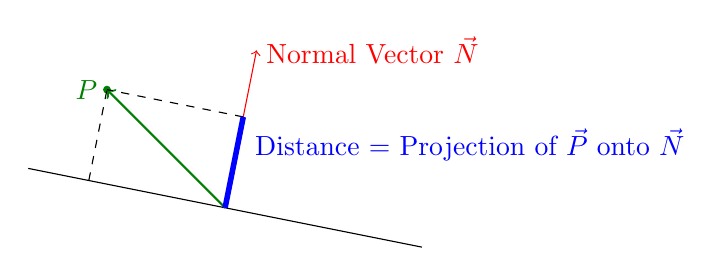
\begin{tikzpicture}
    \draw (0,0) -- (5,-1);
    \draw[red,->] (2.5,-0.5) -- (2.9, 1.5) node[right]{Normal Vector $\vec{N}$};
    \coordinate[label = {[Green]left:$P$}] (P) at (1,1);
    \node at (P) [circle,fill,inner sep=1pt,Green]{};
    \draw[thick,->,Green] (2.5,-0.5) -- (P);
    \draw[dashed] (10/13, -2/13) -- (P);
    \draw[dashed] (71/26, 17/26) -- (P);
    \draw[line width=2pt, blue] (2.5,-0.5) -- (71/26, 17/26) node[below right]{Distance = Projection of $\vec{P}$ onto $\vec{N}$};
    \end{tikzpicture}\\
    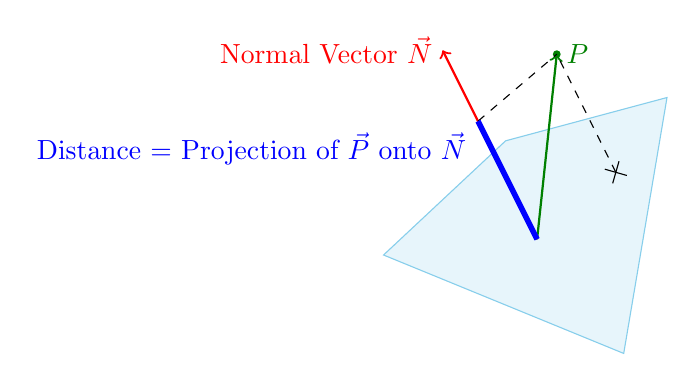
\begin{tikzpicture}[x={(-0.2cm, -0.7cm)}, y={(0.7cm, -0.2cm)}, z={(-0.3cm, 0.6cm)}]
    \filldraw[draw=SkyBlue, fill=SkyBlue!20]
    (0,0,0) -- (2.5,-1.5,0) -- (3,3,0) -- (-1.5,2.5,0) -- cycle;
    \draw[thick,->,red] (1.5,1,0) -- (1.5,1,4) node[left]{Normal Vector $\vec{N}$};
    \coordinate[label = {[Green]right:$P$}] (P) at (0,2,2.5);
    \node at (P) [circle,fill,inner sep=1pt,Green]{};
    \draw[thick,->,Green] (1.5,1,0) -- (P);
    \draw[dashed] (1.5,1,2.5) -- (P);
    \draw[dashed] (0,2,0) -- (P);
    \draw (0,2.2,0) -- (0,1.8,0);
    \draw (0.2,2,0) -- (-0.2,2,0);
    \draw[line width=2pt, blue] (1.5,1,0) -- (1.5,1,2.5) node[below left]{Distance = Projection of $\vec{P}$ onto $\vec{N}$};
    \end{tikzpicture}
    \caption{\textit{Schematic diagram for finding the distance of a point to a line/plane.}}
    \label{fig:distancelp}
\end{figure}

\begin{exmp}
Find the distance from the plane $x-2y+3z = 6$ to the point $(3,3,6)^T$.
\end{exmp}
\begin{solution}
From the equation of the plane, and by Properties \ref{proper:normalhyperplane}, it can be inferred that the normal vector of the plane is $\hat{\imath} - 2\hat{\jmath} + 3\hat{k}$. We can select any point on the plane as we wish, let's say $(4,2,2)^T$, and the vector from such a point to the point $(3,3,6)^T$ in question is simply their difference $(3,3,6)^T - (4,2,2)^T = -\hat{\imath} + \hat{\jmath} + 4\hat{k}$. Subsequently, the distance is found from the length of the projection of this vector $-\hat{\imath} + \hat{\jmath} + 4\hat{k}$ onto the normal vector of the plane $\hat{\imath} - 2\hat{\jmath} + 3\hat{k}$. By (\ref{eqn:scalarproj}) of Properties \ref{proper:proj}, it is
\begin{align*}
\frac{(-\hat{\imath} + \hat{\jmath} + 4\hat{k}) \cdot (\hat{\imath} - 2\hat{\jmath} + 3\hat{k})}{\norm{\hat{\imath} - 2\hat{\jmath} + 3\hat{k}}} = \frac{(-1)(1)+(1)(-2)+(4)(3)}{\sqrt{(1)^2 + (-2)^2 + (3)^2}} = \frac{9}{\sqrt{14}}
\end{align*}
\end{solution}
Sometimes the calculation may lead to a negative value for the projection and we may want to take the absolute value. The case of finding the distance of a point to a line of $\mathbb{R}^3$ is considered in Exercise \ref{ex:dist_pt_line_R3}.

\section{Further Geometric Applications of Cross Product}
Unless specified, all vectors in this section are assumed to be of $\mathbb{R}^3$.
\subsection{Area}
The area of the parallelogram formed by two vectors $\vec{u}$, $\vec{v}$ is simply the absolute value of their cross product, as seen in Figure \ref{fig:crossgeo} below.
\begin{figure}
    \centering
    \begin{tikzpicture}
    \coordinate (0) at (0,0);
    \coordinate (vecu) at (4,0);
    \coordinate (vecv) at (1,3);
    \draw[thick, ->] (0)--(vecu) node[right]{$\vec{u}$};
    \draw[thick, ->] (0)--(vecv) node[above left]{$\vec{v}$};
    \draw[thick, ->, dashed, gray] (4,0)--(5,3);
    \draw[thick, ->, dashed, gray] (1,3)--(5,3);
    \draw[dashed, Green] (1,3)--(4,0);
    \draw[dashed, blue] (1,3)--(1,0) node[pos=0.75, right]{$\norm{\vec{v}}\sin\theta$};
    \draw[red] (1+0.2, 0)--(1+0.2, 0+0.2)--(1, 0+0.2);
    \pic[draw, "$\theta$",angle eccentricity=1.5] {angle = vecu--0--vecv};
    \end{tikzpicture}
    \caption{\textit{Geometric Meaning of the cross product.}}
    \label{fig:crossgeo}
\end{figure}
\begin{proper}
\label{proper:areaparallelogram}
Directly from (\ref{eqn:crossgeo}) of Properties \ref{proper:crossgeo}, the area of the parallelogram formed by two vectors $\vec{u}$ and $\vec{v}$ is
\begin{align}
\norm{\vec{u} \times \vec{v}} = \norm{\vec{u}}\norm{\vec{v}}\sin\theta
\end{align}
Similarly, the area of triangle made by $\vec{u}$ and $\vec{v}$ is half of the above:
\begin{align}
\frac{1}{2}\norm{\vec{u} \times \vec{v}} = \frac{1}{2}\norm{\vec{u}}\norm{\vec{v}}\sin\theta   
\end{align}
\end{proper}

\begin{exmp}
Find the area of the parallelogram formed by $\vec{u} = (-1, -2, 4)^T$ and $\vec{v} = (3, 0, 1)^T$.
\end{exmp}
\begin{solution}
By Formula (\ref{eqn:crossdet}), the cross product between the two given vectors is
\begin{align*}
\vec{u} \times \vec{v} &=
\begin{vmatrix}
\hat{\imath} & \hat{\jmath} & \hat{k} \\
-1 & -2 & 4 \\
3 & 0 & 1
\end{vmatrix} \\
&= -2\hat{\imath} + 13\hat{\jmath} + 6\hat{k}
\end{align*}
Therefore, as suggested by Properties \ref{proper:areaparallelogram}, the required area is
\begin{align*}
\norm{\vec{u} \times \vec{v}} &= \sqrt{(-2)^2 + (13)^2 + (6)^2} \\
&= \sqrt{209}
\end{align*}
\end{solution}

\subsection{Volume}
Meanwhile, the volume of parallelepiped (see Figure \ref{fig:triplevol} below) formed by three vectors $\vec{u}$, $\vec{v}$, $\vec{w}$ is given by the absolute value of the so-called \index{Scalar Triple Product}\keywordhl{scalar triple product} as follows.
\begin{figure}[h!]
    \centering
    \begin{tikzpicture}
\coordinate (0) at (0,0,0);
\fill[fill=orange!20, opacity=0.5] (0) -- (4,0,0) -- (5,0,-2) -- (1,0,-2) -- cycle;
\draw[thick, ->] (0)--(4,0,0) node[right](vecu){$\vec{u}$};
\draw[thick, ->] (0)--(1,0,-2) node[below right](vecv){$\vec{v}$};
\draw[thick, ->] (0)--(1,3,-1) node[above](vecw){$\vec{w}$};
\draw[thick, ->, gray, dashed] (4,0,0)--(5,0,-2);
\draw[thick, ->, gray, dashed] (1,0,-2)--(2,3,-3);
\draw[thick, ->, gray, dashed] (1,3,-1)--(5,3,-1);
\draw[thick, ->, gray, dashed] (4,0,0)--(5,3,-1);
\draw[thick, ->, gray, dashed] (1,0,-2)--(5,0,-2);
\draw[thick, ->, gray, dashed] (1,3,-1)--(2,3,-3);
\draw[thick, ->, gray, dashed] (5,0,-2)--(6,3,-3);
\draw[thick, ->, gray, dashed] (5,3,-1)--(6,3,-3);
\draw[thick, ->, gray, dashed] (2,3,-3)--(6,3,-3);
\draw[blue, dashed] (1,3,-1)--(1,0,-1) node[midway, right]{$\norm{\vec{w}}\cos\theta$};
\draw[blue] (0.9,-0.1,-1) -- (1.1,0.1,-1);
\draw[blue] (0.9,0.1,-1) -- (1.1,-0.1,-1);
\draw[thick, ->, red] (0,0,0) -- (0,3,0) node[above](vecn){$\vec{u}\times\vec{v}$};
\pic[draw, "$\theta$",angle eccentricity=1.75] {angle = vecw--0--vecn};
\draw[orange, <-] (3,0,-1) to [in=190, out=70] (5,2,-1) node[right]{Base Area $= \norm{\vec{u}\times\vec{v}}$};
\end{tikzpicture}
    \caption{\textit{The relationship between the volume of parallelepiped and its scalar triple product.}}
    \label{fig:triplevol}
\end{figure}
\begin{proper}[Scalar Triple Product]
\label{proper:parallelpiped}
The volume of parallelepiped formed by three vectors $\vec{u}$, $\vec{v}$, and $\vec{w}$ is calculated as
\begin{align}
\norm{\vec{u} \times \vec{v}} \norm{\vec{w}} \cos\theta = |(\vec{u} \times \vec{v}) \cdot \vec{w}| =
\text{abs}\left(
\begin{vmatrix}
u_1 & u_2 & u_3 \\
v_1 & v_2 & v_3 \\
w_1 & w_2 & w_3
\end{vmatrix}\right) \label{eqn:scalartriple}
\end{align}
where
\begin{align}
(\vec{u} \times \vec{v}) \cdot \vec{w} =
\begin{vmatrix}
u_1 & u_2 & u_3 \\
v_1 & v_2 & v_3 \\
w_1 & w_2 & w_3
\end{vmatrix}    
\end{align}
is the scalar triple product of $\vec{u}$, $\vec{v}$, and $\vec{w}$. Also, by applying Properties \ref{proper:elementaryopdet}, the determinant form of the scalar triple product indicates that
\begin{align}
\begin{aligned}
&\quad (\vec{u} \times \vec{v}) \cdot \vec{w} = (\vec{v} \times \vec{w}) \cdot \vec{u} = (\vec{w} \times \vec{u}) \cdot \vec{v} \\
&= -(\vec{v} \times \vec{u}) \cdot \vec{w} = -(\vec{w} \times \vec{v}) \cdot \vec{u} = -(\vec{u} \times \vec{w}) \cdot \vec{v}    
\end{aligned}
\end{align}
\end{proper}
\begin{proof}
We will prove the determinant formula shown above for $(\vec{u} \times \vec{v}) \cdot \vec{w}$ briefly. By Formula (\ref{eqn:crossdet}) from Properties \ref{proper:crossdet}, we have
\begin{align*}
\vec{u} \times \vec{v} &= (u_2v_3 - u_3v_2)\hat{\imath} + (u_3v_1 - u_1v_3)\hat{\jmath} + (u_1v_2 - u_2v_1)\hat{k}     
\end{align*}
and then according to Definition \ref{defn:dotreal}
\begin{align*}
(\vec{u} \times \vec{v}) \cdot \vec{w} &= (u_2v_3 - u_3v_2, u_3v_1 - u_1v_3, u_1v_2 - u_2v_1)^T \cdot (w_1, w_2, w_3)^T \\ 
&= (u_2v_3 - u_3v_2)(w_1) + (u_3v_1 - u_1v_3)(w_2) + (u_1v_2 - u_2v_1)(w_3) 
\end{align*}
which is equal to
\begin{align*}
\begin{vmatrix}
u_1 & u_2 & u_3 \\
v_1 & v_2 & v_3 \\
w_1 & w_2 & w_3
\end{vmatrix}
= w_1(u_2v_3 - u_3v_2) - w_2(u_1v_3 - u_3v_1) + w_3(u_1v_2 - u_2v_1) 
\end{align*}
where we do cofactor expansion (Properties \ref{proper:cofactorex}) along the third row of the determinant.
\end{proof}
If the volume of the parallelepiped evaluated from the scalar triple product is zero, it implies that the three vectors involved are \index{Co-planar}\keywordhl{co-planar}, i.e.\ lying on the same plane.
\begin{proper}
Given three vectors $\vec{u}$, $\vec{v}$, and $\vec{w}$, if their scalar triple product $(\vec{u} \times \vec{v}) \cdot \vec{w} = 0$ equals zero, then $\vec{u}$, $\vec{v}$, and $\vec{w}$ are co-planar and lie on the same plane, and vice versa.
\end{proper}
Note that if $\vec{w} = \alpha \vec{u} + \beta \vec{v}$, where $\alpha$ and $\beta$ are some scalars, then $\vec{u}$, $\vec{v}$, $\vec{w}$ are co-planar, and $(\vec{u} \times \vec{v}) \cdot \vec{w} = (\vec{u} \times \vec{v}) \cdot (\alpha \vec{u} + \beta \vec{v}) = \alpha ((\vec{u} \times \vec{v}) \cdot \vec{u}) + \beta ((\vec{u} \times \vec{v}) \cdot \vec{v}) = \alpha(0) + \beta(0) = 0$ as both $\vec{u} \cdot (\vec{u} \times \vec{v})$ and $\vec{v} \cdot (\vec{u} \times \vec{v})$ equal to zero (why?).

\begin{exmp}
Find the volume of the parallelepiped formed by $\vec{u} = (1,-2,2)^T$, $\vec{v}=(-1,-1,1)^T$ and $\vec{w}=(2,1,0)^T$.
\end{exmp}
\begin{solution}
By Properties \ref{proper:parallelpiped}, the triple scalar product of the three given vectors is
\begin{align*}
(\vec{u} \times \vec{v}) \cdot \vec{w} &=
\begin{vmatrix}
1 & -2 & 2 \\
-1 & -1 & 1 \\
2 & 1 & 0
\end{vmatrix}
= -3
\end{align*}
and the volume is $\abs{-3} = 3$.
\end{solution}

\subsubsection{Generalization to other dimensions}
Given that the volume of parallelepiped formed by three vectors is equal to the absolute value of the corresponding matrix determinant as derived above, it is natural to ask if similar results hold for other numbers of dimension. In fact, Properties \ref{proper:parallelpiped} can be generalized to include length, area, and the so-called \textit{$n$-volume} (Volume equivalent of $n$ vectors in the $n$-dimensional space).
\begin{proper}
\label{proper:nvolume}
For $n$ vectors of $\mathbb{R}^n$, their $n$-volume is the absolute value of the determinant of the matrix formed by these column (or row) vectors. When $n=1,2,3$, the $n$-volume corresponds to the usual notions of length, area, and volume.
\end{proper}
We can check the legitimacy of the last sentence in Properties \ref{proper:nvolume} by noticing that it is consistent with Properties \ref{proper:areaparallelogram} about the area of two vectors on the $xy$ plane. Given $\vec{u} = (u_1, u_2)^T$ and $\vec{v} = (v_1, v_2)^T$, by Properties \ref{proper:nvolume} the area of the parallelogram formed by them will be
\begin{align*}
\begin{vmatrix}
u_1 & u_2 \\
v_1 & v_2
\end{vmatrix} = u_1v_2 - v_1u_2
\end{align*}
Alternatively, we can treat $\vec{u}$ and $\vec{v}$ as two three-dimensional vectors $(u_1, u_2, 0)^T$ and $(v_1, v_2, 0)^T$ such that they have a zero $z$-component and remain lying on the $xy$ plane. Then according to the previous Properties \ref{proper:areaparallelogram}, the area is computed as $\norm{\vec{u} \times \vec{v}}$, and by Properties \ref{proper:crossdet} it is
\begin{align*}
\vec{u} \times \vec{v} &= 
\begin{vmatrix}
\hat{\imath} & \hat{\jmath} & \hat{k} \\
u_1 & u_2 & 0 \\
v_1 & v_2 & 0
\end{vmatrix} \\
&= \hat{k}\begin{vmatrix}
u_1 & u_2 \\
v_1 & v_2
\end{vmatrix} \quad \text{(Cofactor Expansion along the third row)}\\
&= (u_1v_2 - v_1u_2)\hat{k} = (0,0,u_1v_2 - v_1u_2)^T
\end{align*}
Hence $\norm{\vec{u} \times \vec{v}} = \sqrt{(0)^2 + (0)^2 + (u_1v_2 - v_1u_2)^2} = u_1v_2 - v_1u_2$, which coincides with the expression we just derived from Properties \ref{proper:nvolume}.

\subsubsection{Remarks}
The solution of a linear system can be considered as a point/line/plane/hyperplane too, depending on the number of free variables and thus direction vectors in the complementary part ($0$/$1$/$2$ or more). We may also like to call it a \textit{solution space}. However, while such shapes surely occupy space geometrically, we have been shying away from defining what really means by a \textit{vector space} mathematically, which will be the main point of discussion in the next chapter.

\section{Useful Vector Identities}
In this section, we will prove some key vector identities that may be of utility to some readers.
\begin{proper}[Vector Triple Product]
\label{proper:triplecross}
The \index{Vector Triple Product}\keywordhl{vector triple product} of three vectors $\vec{u}$, $\vec{v}$, $\vec{w}$ is defined as
\begin{align}
\vec{u} \times (\vec{v} \times \vec{w}) = (\vec{u} \cdot \vec{w})\vec{v} - (\vec{u} \cdot \vec{v})\vec{w}
\label{eqn:triplecross}
\end{align}
\end{proper}
\begin{proof}
By Properties \ref{proper:crossdet}, the L.H.S. can be expanded into
\begin{align*}
&\quad\vec{u} \times (\vec{v} \times \vec{w}) \\
&= (u_1\hat{\imath} + u_2\hat{\jmath} + u_3\hat{k}) \\
&\quad \times [(v_2w_3 - v_3w_2)\hat{\imath} + (v_3w_1 - v_1w_3)\hat{\jmath} + (v_1w_2 - v_2w_1)\hat{k}] \\
&= 
\begin{vmatrix}
\hat{\imath} & \hat{\jmath} & \hat{k} \\
u_1 & u_2 & u_3 \\
v_2w_3 - v_3w_2 & v_3w_1 - v_1w_3 & v_1w_2 - v_2w_1 
\end{vmatrix}
\end{align*}
The $\hat{\imath}$ component along the $x$-direction is
\begin{align*}
&\quad u_2(v_1w_2 - v_2w_1) - u_3(v_3w_1 - v_1w_3) \\
&= u_2w_2v_1 + u_3w_3v_1 - u_2v_2w_1 - u_3v_3w_1 \\
&= u_1w_1v_1 + u_2w_2v_1 + u_3w_3v_1 - u_1v_1w_1 - u_2v_2w_1 - u_3v_3w_1 \\
&= (u_1w_1 + u_2w_2 + u_3w_3)v_1 - (u_1v_1 + u_2v_2 + u_3v_3)w_1 \\
&= (\vec{u} \cdot \vec{w})v_1 - (\vec{u} \cdot \vec{v})w_1
\end{align*}
which is equal to the $\hat{\imath}$ component on the R.H.S. and similar results can be shown for the $\hat{\jmath}$, $\hat{k}$ components and the equality establishes.
\end{proof}

\begin{proper}[Jacobi Identity]
\begin{align}
\vec{u} \times (\vec{v} \times \vec{w}) + \vec{v} \times (\vec{w} \times \vec{u}) + \vec{w} \times (\vec{u} \times \vec{v}) = \textbf{0}    
\end{align}
\end{proper}
\begin{proof}
By Properties \ref{proper:triplecross}, we have
\begin{align*}
&\quad \vec{u} \times (\vec{v} \times \vec{w}) + \vec{v} \times (\vec{w} \times \vec{u}) + \vec{w} \times (\vec{u} \times \vec{v}) \\
&= [(\vec{u} \cdot \vec{w})\vec{v} - (\vec{u} \cdot \vec{v})\vec{w}] \\
&\quad + [(\vec{v} \cdot \vec{u})\vec{w} - (\vec{v} \cdot \vec{w})\vec{u}] \\
&\quad + [(\vec{w} \cdot \vec{v})\vec{u} - (\vec{w} \cdot \vec{u})\vec{v}] \\
&= [(\vec{u} \cdot \vec{w})\vec{v} - (\vec{w} \cdot \vec{u})\vec{v}] \\
&\quad + [(\vec{v} \cdot \vec{u})\vec{w} - (\vec{u} \cdot \vec{v})\vec{w}] \\
&\quad + [(\vec{w} \cdot \vec{v})\vec{u} - (\vec{v} \cdot \vec{w})\vec{u}] \\
&= 0\vec{v} + 0\vec{w} + 0\vec{u} = \textbf{0}
\end{align*}
\end{proof}

\begin{proper}[Lagrange's Identity]
\begin{align}
\norm{\vec{u} \times \vec{v}}^2 = \norm{\vec{u}}^2 \norm{\vec{v}}^2 - (\vec{u} \cdot \vec{v})^2
\end{align}
\end{proper}
\begin{proof}
Manipulating the geometric formulae of dot/cross product, we have
\begin{align*}
\norm{\vec{u} \times \vec{v}}^2 &= \norm{\vec{u}}^2 \norm{\vec{v}}^2 \sin^2 \theta  &\text{(Properties \ref{proper:crossgeo})} \\
&= \norm{\vec{u}}^2 \norm{\vec{v}}^2 (1 - \cos^2 \theta) \\
&= \norm{\vec{u}}^2 \norm{\vec{v}}^2 - \norm{\vec{u}}^2 \norm{\vec{v}}^2 \cos^2 \theta \\
&= \norm{\vec{u}}^2 \norm{\vec{v}}^2 - (\vec{u} \cdot \vec{v})^2 &\text{(Properties \ref{proper:dotgeo})}
\end{align*}
\end{proof}

The last identity is the \index{Cosine Law for Spherical Trigonometry}\keywordhl{Cosine Law for Spherical Trigonometry}.
\begin{proper}[Cosine Law for Spherical Trigonometry]
\label{proper:cosinesphere}
\begin{align}
\cos c = \cos a \cos b + \sin a \sin b \cos C    
\end{align}
where $a$, $b$, $c$ are the (subtended angle of) three arcs (in radians) of a spherical triangle on a unit sphere and $C$ is the angle between the two arcs $a$ and $b$, as shown in Figure \ref{fig:cosinesphere}.
\end{proper}
\begin{figure}
\centering\tdplotsetmaincoords{35}{125}
% https://tex.stackexchange.com/questions/380316/gray-shaded-sphere-with-tikz-3dplot
% https://latexdraw.com/draw-a-sphere-in-latex-using-tikz/#t-1610955504379
\begin{tikzpicture}[scale=2.5,tdplot_main_coords]
    % spherical background
    \draw [ball color=white,very thin] (0,0,0) circle (1cm) ;
    % equator
    \coordinate (0) at (0,0,0);
    % spherical triangle
    \begin{scope}[rotate=15]
    \tdplotdefinepoints(0,0,1)(0,0.1,0.99)(0.1,0,0.99)
    \tdplotdrawpolytopearc[thick, purple]{0.15}{below, purple}{$C$}
    \tdplotdefinepoints(0,0,0)(0,0,1)(3^0.5/2,0,0.5)
    \tdplotdrawpolytopearc[thick, red]{1}{left, red}{$a$}
    \tdplotdefinepoints(0,0,0)(0,0,1)(0,0.8,0.6)
    \tdplotdrawpolytopearc[thick, blue]{1}{above, blue}{$b$}
    \tdplotdefinepoints(0,0,0)(0,0.8,0.6)(3^0.5/2,0,0.5)
    \tdplotdrawpolytopearc[thick, Green]{1}{below, Green}{$c$}
    \draw[dashed, color=black!60] (0,0,0) -- (0,0,1) node(C){};
    \draw[dashed, color=black!60] (0,0,0) -- (3^0.5/2,0,0.5) node(B){};
    \draw[dashed, color=black!60] (0,0,0) -- (0,0.8,0.6) node(A){};
    \end{scope}
\end{tikzpicture}
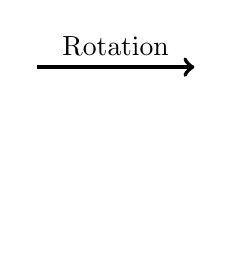
\begin{tikzpicture}
    \draw[line width=1.5, ->] (0,2) -- (2,2) node[midway,above]{Rotation};
    \node at (0,0){};
\end{tikzpicture}
\tdplotsetmaincoords{80}{115}
% https://tex.stackexchange.com/questions/380316/gray-shaded-sphere-with-tikz-3dplot
\begin{tikzpicture}[scale=2.5,tdplot_main_coords]
    % spherical background
    \draw [ball color=white,very thin] (0,0,0) circle (1cm) ;
    % equator
    \coordinate (0) at (0,0,0);
    % spherical triangle
    \tdplotsetrotatedcoords{90}{90}{90};
    \draw[orange, dashed,
        tdplot_rotated_coords] (0,1,0) arc (90:252:1) node[orange, pos=0.84, right, align=left, font=\scriptsize]{Prime \\ Meridian \\};
    \tdplotdefinepoints(0,0,0)(0,0,1)(0,0.6,-0.8)
    \tdplotdrawpolytopearc[dashed, color=white]{1}{}{}
    \draw[dashed, ->, color=black!60] (0,0,0) -- (0,0,1) node(C){};
    \draw[dashed, ->, color=black!60] (0,0,0) -- (3^0.5/2,0,0.5) node(B)[black, font=\tiny, pos=0.75, sloped, below]{$\hat{v} = (\sin a, 0, \cos a)$};
    \draw[dashed, ->, color=black!60] (0,0,0) -- (0,0.8,0.6) node(A)[black, font=\tiny, pos=0.35, sloped, below]{$\hat{w} = (\sin b \cos C, \sin b \sin C, \cos b)$};
    \tdplotdefinepoints(0,0,0)(0,0,1)(3^0.5/2,0,0.5)
    \tdplotdrawpolytopearc[thick, red]{1}{left, red}{$a$}
    \tdplotdefinepoints(0,0,0)(0,0,1)(0,0.8,0.6)
    \tdplotdrawpolytopearc[thick, blue]{1}{below, blue}{$b$}
    \tdplotdefinepoints(0,0,0)(0,0.8,0.6)(3^0.5/2,0,0.5)
    \tdplotdrawpolytopearc[thick, Green]{1}{below, Green}{$c$}
    \node at (0,0.04,0.88)[purple]{$C$};
    \node at (0,0,1.15)[align=left, font=\scriptsize]{North Pole \\ $\hat{u} = (0,0,1)$};
\end{tikzpicture}
\caption{\textit{The spherical triangle on a unit sphere as described in Properties \ref{proper:cosinesphere}.}}
\label{fig:cosinesphere}
\end{figure}
\begin{proof}
For the given spherical triangle, we can always rotate the coordinate system (see Figure \ref{fig:cosinesphere}) while keeping its shape intact, such that the corner $C$ is positioned exactly at the north pole ($\hat{u} = (0,0,1)^T$) and one of the two arcs starting from corner $C$ (let's say $a$) lies along the Prime Meridian (angle from the $x$-axis is $\SI{0}{\degree}$, i.e. $y = 0$). The vector $\hat{v}$ at the end of arc $a$ will then have a direction of $(\sin a, 0, \cos a)^T$. The vector $\hat{w}$ to the remaining corner at the intersection of arcs $b$ and $c$ will similarly have a $z$-component of $\cos b$, and its projection on the $xy$ plane will be $\sin b$ and the $x$/$y$-component will then be $\sin b \cos C$ and $\sin b \sin C$, i.e. $\hat{w} = (\sin b \cos C, \sin b \sin C, \cos b)^T$. \par
Now consider the dot product $\hat{v} \cdot \hat{w}$. The geometric meaning of dot product (Properties \ref{proper:dotgeo}) implies that it is the angle between $\hat{v}$ and $\hat{w}$, that is, $\hat{v} \cdot \hat{w} = \cos c$. On the other hand,
\begin{align*}
\hat{v} \cdot \hat{w} &= (\sin a, 0, \cos a)^T \cdot (\sin b \cos C, \sin b \sin C, \cos b)^T \\
&= (\sin a) (\sin b \cos C) + (0) (\sin b \sin C) + (\cos a) (\cos b) \\
&= \cos a \cos b + \sin a \sin b \cos C 
\end{align*}
Therefore, equaling the two expressions of $\hat{v} \cdot \hat{w}$ gives the desired formula of $\cos c = \cos a \cos b + \sin a \sin b \cos C$.
\end{proof}

\section{Earth Science Applications}
\begin{exmp}
\label{exmp:Haversine}
Derive the \textit{Haversine Formula} for finding the great-circle distance between any two points on a sphere with their latitudes/longitudes provided. Hence find the distance between New York (\SI{40.73}{\degree N}, \SI{73.94}{\degree W}) and Warsaw (\SI{52.24}{\degree N}, \SI{21.02}{\degree E}).
\end{exmp}
\begin{solution}
Denote the latitudes/longitudes of the two locations by $\varphi_{1,2}$ and $\lambda_{1,2}$. Starting from the Cosine Law for Spherical Trigonometry (Properties \ref{proper:cosinesphere}) with corner $C$ still fixed at north pole but arc $a$ not necessarily along the Prime Meridian, we have $C = \lambda_2 - \lambda_1$, $a = \frac{\pi}{2} - \varphi_1$, $b = \frac{\pi}{2} - \varphi_2$, and
\begin{align*}
\cos c &= \cos a \cos b + \sin a \sin b \cos C \\
\cos c &= \cos (\frac{\pi}{2} - \varphi_1) \cos (\frac{\pi}{2} - \varphi_2) + \sin (\frac{\pi}{2} - \varphi_1) \sin (\frac{\pi}{2} - \varphi_2) \cos (\lambda_2 - \lambda_1) \\
\cos c &= \sin \varphi_1 \sin \varphi_2 + \cos \varphi_1 \cos \varphi_2 \cos (\lambda_2 - \lambda_1)
\end{align*}
The \textit{haversine} of an angle $\theta$ is $\text{hav}(\theta) = \sin^2 (\frac{\theta}{2}) = \frac{1}{2}(1-\cos\theta)$ and therefore $\cos\theta = 1 - 2\ \text{hav}(\theta)$. Subsequently,
\begin{align}
\cos c &= \sin \varphi_1 \sin \varphi_2 + \cos \varphi_1 \cos \varphi_2 (1 - 2\ \text{hav}(\lambda_2 - \lambda_1)) \nonumber \\ 
\cos c &= \sin \varphi_1 \sin \varphi_2 + \cos \varphi_1 \cos \varphi_2 - 2 \cos \varphi_1 \cos \varphi_2\ \text{hav}(\lambda_2 - \lambda_1) \nonumber \\
\cos c &= \cos(\varphi_2 - \varphi_1) - 2 \cos \varphi_1 \cos \varphi_2\ \text{hav}(\lambda_2 - \lambda_1) \nonumber \\
(1 - 2\ \text{hav}(c)) &= (1 - 2\ \text{hav}(\varphi_2 - \varphi_1)) - 2 \cos \varphi_1 \cos \varphi_2\ \text{hav}(\lambda_2 - \lambda_1) \nonumber \\
\text{hav}(c) &= \text{hav}(\varphi_2 - \varphi_1) + \cos \varphi_1 \cos \varphi_2\ \text{hav}(\lambda_2 - \lambda_1)
\end{align}
where we have used the trigonometric identity $\cos(\theta-\phi) = \cos \theta \cos \phi + \sin \theta \sin \phi$ in the middle. The \textit{Haversine Formula} is now established and we can use it to calculate the angle $c$ subtended by the arc between two locations and hence their distance by $d = Rc$ where $R$ is the radius (of the Earth, \SI{6370}{\km}). For New York (\SI{40.73}{\degree N}, \SI{73.94}{\degree W}) and Warsaw (\SI{52.24}{\degree N}, \SI{21.02}{\degree E}), $\lambda_1 = \SI{-73.94}{\degree}$, $\lambda_2 = \SI{21.02}{\degree}$, $\varphi_1 = \SI{40.73}{\degree}$, $\varphi_2 = \SI{52.24}{\degree}$, and
\begin{align*}
\text{hav}(c) &= \text{hav}(\SI{52.24}{\degree} - \SI{40.73}{\degree}) \\
&\quad+ \cos (\SI{40.73}{\degree}) \cos (\SI{52.24}{\degree})\ \text{hav}(\SI{21.02}{\degree} - (\SI{-73.94}{\degree})) \\
&= \text{hav}(\SI{11.51}{\degree}) + \cos (\SI{40.73}{\degree}) \cos (\SI{52.24}{\degree})\ \text{hav}(\SI{94.96}{\degree}) \\
&= \sin^2 (\frac{\SI{11.51}{\degree}}{2}) + \cos (\SI{40.73}{\degree}) \cos (\SI{52.24}{\degree}) \sin^2 (\frac{\SI{94.96}{\degree}}{2}) \\
\sin^2 (\frac{c}{2}) &\approx 0.26214 \\
c &\approx \SI{61.6}{\degree} = \SI{1.075}{\radian}
\end{align*}
and therefore the required distance is $d = Rc = (\SI{6370}{\km})(\SI{1.075}{\radian}) \approx \SI{6848}{\km}$. The value computed by the Haversine Formula will be slightly off from the true value since the Earth is not a perfect sphere but rather an oblate one.
\end{solution}

\begin{exmp}
The Earth's magnetic field can be approximated by a magnetic dipole so that the magnetic field lines on the Earth's surface are oriented from the geomagnetic North Pole to the geomagnetic South Pole (like longitudinal lines but for the geomagnetic dipole). In 2020, the geomagnetic North Pole is at \SI{80.7}{\degree N}, \SI{72.7}{\degree W}. Find the magnetic declination (angle from the geographic North to geomagnetic North) at Tokyo (\SI{35.65}{\degree N}, \SI{139.84}{\degree E}) according to this \textit{geomagnetic dipole model}.
\end{exmp}
\begin{solution}
To find the magnetic declination we need to calculate the three arcs of the spherical triangle with its three corners at the geographic/geomagnetic North Pole and Tokyo. The arc distance between geographic/geomagnetic North Pole $d$ is simply $\SI{90}{\degree} - \SI{80.7}{\degree} = \SI{9.3}{\degree}$. Similarly, the arc from the geographic North Pole to Tokyo is $a = \SI{90}{\degree} - \SI{35.65}{\degree} = \SI{54.35}{\degree}$. We can use the Haversine Formula derived in the last example to obtain the arc from the geomagnetic North Pole to Tokyo, which yields
\begin{align*}
\text{hav}(t) &= \text{hav}(\SI{80.7}{\degree} - \SI{35.65}{\degree}) \\ 
&\quad + \cos(\SI{35.65}{\degree}) \cos(\SI{80.7}{\degree})\ \text{hav}((\SI{-72.7}{\degree}) - \SI{139.84}{\degree}) \\
&= \text{hav}(\SI{45.05}{\degree}) + \cos(\SI{35.65}{\degree}) \cos(\SI{80.7}{\degree})\ \text{hav}(\SI{-212.54}{\degree}) \\
&\approx 0.26777 \\
t &\approx \SI{62.3}{\degree}
\end{align*}
Denote the declination angle by $D$. By Properties \ref{proper:cosinesphere}, we have
\begin{align*}
\cos d &= \cos a \cos t + \sin a \sin t \cos D \\
\cos (\SI{9.3}{\degree}) &= \cos (\SI{54.35}{\degree}) \cos (\SI{62.3}{\degree}) + \sin (\SI{54.35}{\degree}) \sin (\SI{62.3}{\degree}) \cos D \\
\cos D &\approx 0.9951 \\
D &\approx \pm \SI{5.7}{\degree}
\end{align*}
To determine the sign, we note that concluded from the longitudes of Tokyo and the geomagnetic North, the geomagnetic North is located to the east of Tokyo, and hence $D = \SI{5.7}{\degree E}$. However, we note that the actual declination is \SI{7.8}{\degree W} which has an opposite sign and is far from our answer (you can extract the value from \href{https://www.ngdc.noaa.gov/geomag/calculators/magcalc.shtml}{https://www.ngdc.noaa.gov/geomag/calculators/magcalc.shtml}). The reason is that the geomagnetic dipole is only a rough first-order approximation, while in reality the Earth's magnetic field has a much more complex structure.
\end{solution}

\section{Python Programming}
Projection as in Properties \ref{proper:proj} can be calculated by \verb|numpy| functions and let's wrap them up in our self-defined function as below.
\begin{lstlisting}
def scalar_projection(u, v):
    """ Calculates the scalar projection of v onto u. """
    return np.dot(u,v) / np.linalg.norm(u)
\end{lstlisting}
This computes the scalar projection of $\vec{v}$ onto $\vec{u}$. Testing with Example \ref{exmp:projectuv} shows 
\begin{lstlisting}
u = np.array([4., 1., -3.])
v = np.array([-2., 3., -1.])
print(scalar_projection(u, v))    
\end{lstlisting}
a consistent output of \texttt{-0.39223}. Incorporating the unit vector function (\verb|unit_vector()|) defined in the last chapter's programming section, we obtain the vector projection.
\begin{lstlisting}
def vector_projection(u, v):
    """ Calculates the vector projection of v onto u. """
    return scalar_projection(u, v) * unit_vector(u)

print(vector_projection(u, v))    
\end{lstlisting}
This results in \texttt{[-0.3077 -0.0769  0.2308]} which matches the example's answer. The area of parallelogram formed by two vectors is the magnitude of their cross product and the corresponding function is typed below.
\begin{lstlisting}
def area_parallelogram(u, v):
    """ Calculate the area of parallelogram formed by two vectors u and v. """
    return np.linalg.norm(np.cross(u,v))
\end{lstlisting}
\verb|print(area_parallelogram(u, v))| then gives \texttt{18.974}. Meanwhile, the function to compute the volume of parallelepiped made up of three vectors can be defined such that it uses the determinant formula in Properties \ref{proper:parallelpiped}.
\begin{lstlisting}
def volume_parallelepiped(u, v, w):
    """ Calculate the volume of parallelepiped formed by two vectors u, v, w. """
    return np.abs(np.linalg.det(np.c_[u,v,w]))

w = np.array([1., 2., -3.])
print(volume_parallelepiped(u, v, w))
\end{lstlisting}
(\verb|np.c_[]| is a shorthand of combining arrays column by column) produces \texttt{14.00000...04} due to numerical round-off error (the true answer would be just $14$). Finally, let's conclude this section by defining the Haversine Formula in Example \ref{exmp:Haversine}.
\begin{lstlisting}
def Haversine_dist(latlon1, latlon2):
    """ Haversine Formula for computing the great-circle 
        distance between two places on the Earth. 
        Input: (lat1, lon1), (lat2, lon2) in degrees.
        Output: Great-circle distance in km.
    """
    R_Earth = 6370 # Earth's Radius
    lat1, lon1 = latlon1[0], latlon1[1]
    lat2, lon2 = latlon2[0], latlon2[1]
    # Converting degree to radian
    lat1_rad, lon1_rad, lat2_rad, lon2_rad = np.deg2rad(lat1), np.deg2rad(lon1), np.deg2rad(lat2), np.deg2rad(lon2) 
    # Haversine's Formula
    hav_c = np.sin((lat2_rad-lat1_rad)/2)**2 + np.cos(lat1_rad)*np.cos(lat2_rad)*np.sin((lon2_rad-lon1_rad)/2)**2 
    arc_c = 2*np.arcsin(np.sqrt(hav_c)) # Inverting to get the great-circle arc angle
    return(R_Earth*arc_c) # Arc angle to arc length
\end{lstlisting}
Using the latitudes and longitudes of New York and Warsaw in Example \ref{exmp:Haversine} for testing, \verb|Haversine_dist((40.73, -73.94), (52.24, 21.02))| outputs \texttt{6847.76}.

\section{Exercises}

\begin{Exercise}
Parameterize the following equations into vector form.
\begin{enumerate}[label=(\alph*)]
\item $6x + 8y = 9$,
\item $x + 9y + 9z = 7$,
\item $y = 3, -\infty < x < \infty$, and
\item $2x + z = 9, -\infty < y < \infty$.
\end{enumerate}
\end{Exercise}
\begin{Answer}
\begin{enumerate}[label=(\alph*)]
\item
$\begin{bmatrix}
x\\
y    
\end{bmatrix}
=
\begin{bmatrix}
\frac{3}{2}\\
0
\end{bmatrix}
+
t
\begin{bmatrix}
-\frac{4}{3}\\
1
\end{bmatrix}
$
\item
$\begin{bmatrix}
x\\
y\\
z
\end{bmatrix}
=
\begin{bmatrix}
7\\
0\\
0
\end{bmatrix}
+
s
\begin{bmatrix}
-9\\
1\\
0
\end{bmatrix}
+
t
\begin{bmatrix}
-9\\
0\\
1
\end{bmatrix}
$
\item 
$\begin{bmatrix}
x\\
y
\end{bmatrix}
=
\begin{bmatrix}
0\\
3
\end{bmatrix}
+
t
\begin{bmatrix}
1\\
0
\end{bmatrix}
$
\item
$\begin{bmatrix}
x\\
y\\
z
\end{bmatrix}
=
\begin{bmatrix}
\frac{9}{2}\\
0\\
0
\end{bmatrix}
+
s
\begin{bmatrix}
0\\
1\\
0
\end{bmatrix}
+
t
\begin{bmatrix}
-\frac{1}{2}\\
0\\
1
\end{bmatrix}$
\end{enumerate}
\end{Answer}

\begin{Exercise}
Eliminate the parameters and find the direct equation.
\begin{enumerate}[label=(\alph*)]
\item \begin{align*}
\begin{bmatrix}
x\\
y
\end{bmatrix}
=
\begin{bmatrix}
2\\
9
\end{bmatrix}
+
t
\begin{bmatrix}
1\\
1
\end{bmatrix}
\end{align*}
\item \begin{align*}
\begin{bmatrix}
x\\
y\\
z
\end{bmatrix}
=
\begin{bmatrix}
6\\
3\\
2
\end{bmatrix}
+
s
\begin{bmatrix}
7\\
4\\
1
\end{bmatrix}
+
t
\begin{bmatrix}
8\\
0\\
5
\end{bmatrix}
\end{align*}
\end{enumerate}
where $-\infty < s,t < \infty$.
\end{Exercise}
\begin{Answer}
\begin{enumerate}[label=(\alph*)]
\item
Normal vector to the line is 
$\begin{bmatrix}
1\\
-1
\end{bmatrix}
$.\\
Equation: $\begin{bmatrix}
1\\
-1
\end{bmatrix}
\cdot
\begin{bmatrix}
x\\
y
\end{bmatrix}
=
\begin{bmatrix}
1\\
-1
\end{bmatrix}
\cdot
\begin{bmatrix}
2\\
9
\end{bmatrix}
\rightarrow
x - y = -7$
\item
Normal vector to the plane is 
$\begin{bmatrix}
7\\
4\\
1
\end{bmatrix}
\times
\begin{bmatrix}
8\\
0\\
5
\end{bmatrix}
=
\begin{bmatrix}
20\\
-27\\
-32
\end{bmatrix}
$.\\
Equation:
$\begin{bmatrix}
20\\
-27\\
-32\\
\end{bmatrix}
\cdot
\begin{bmatrix}
x\\
y\\
z
\end{bmatrix}
=
\begin{bmatrix}
20\\
-27\\
-32\\
\end{bmatrix}
\cdot
\begin{bmatrix}
6\\
3\\
2
\end{bmatrix}
\rightarrow
20x - 27y - 32z = -25$
\end{enumerate}
\end{Answer}

\begin{Exercise}
\label{ex:dist_pt_line_R3}
Find the distance of the point $(3,2,9)^T$ to the plane $x + 2y + 5z = 10$, as well as the distance of the point $(3,2,9)^T$ to the line 
\begin{align*}
\begin{bmatrix}
x\\
y\\
z
\end{bmatrix}
=
t
\begin{bmatrix}
0\\
1\\
2
\end{bmatrix}
\end{align*}
where $-\infty < t < \infty$.
\end{Exercise}
\begin{Answer}
Part 1: Choose $(0,0,2)^T$ as a reference point on the plane.\\
Projection of the vector from $(0,0,2)^T$ to $(3,2,9)^T$: $(3-0)\hat{\imath} + (2-0)\hat{\jmath} + (9-2)\hat{k} = 3\hat{\imath} + 2\hat{\jmath} + 7\hat{k}$ onto the normal vector $\hat{\imath} + 2\hat{\jmath} + 5\hat{k}$ of the plane is
\[\frac{(3)(1)+(2)(2)+(7)(5)}{\sqrt{1^2 + 2^2 + 5^2}} = \frac{42}{\sqrt{30}}\] which is the required distance.\\
Part 2: Choose $(0,1,2)^T$ as a reference point along the line. Find the projection of $(3,2,9)^T - (0,1,2)^T = 3\hat{\imath} + 1\hat{\jmath} + 7\hat{k}$ onto the direction vector $\hat{\jmath} + 2\hat{k}$, which is
\begin{align*}
\frac{(3)(0)+(1)(1)+(7)(2)}{0^2 + 1^2 + 2^2} (\hat{\jmath} + 2\hat{k}) &= 3(\hat{\jmath} + 2\hat{k}) = 3\hat{\jmath} + 6\hat{k}
\end{align*}
The displacement vector between the point and line (which is orthogonal to the line) is then $(3\hat{\imath} + 1\hat{\jmath} + 7\hat{k}) - (3\hat{\jmath} + 6\hat{k}) = 3\hat{\imath} - 2\hat{\jmath} + \hat{k}$ and the required distance equals to $\sqrt{3^2 + (-2)^2 + 1^2} = \sqrt{14}$.
\end{Answer}

\begin{Exercise}
Prove that the shortest distance between two lines, $\vec{u} = \vec{a} + s\hat{l}$ and $\vec{v} = \vec{b} + t\hat{m}$, where $-\infty < s,t < \infty$, $\vec{a}, \vec{b}$ are some arbitrary vectors and $\hat{l}, \hat{m}$ are some fixed, non-parallel unit vectors representing direction of the two lines, is
\begin{align*}
\text{Dist}(\vec{u}, \vec{v}) = \frac{(\hat{a}-\hat{b}) \cdot (\hat{l} \times \hat{m})}{\norm{\hat{l} \times \hat{m}}}
\end{align*}
Hints: Geometrically, the distance between these two lines is the projection of any vector from one line to another onto the vector normal to the plane made by $\hat{l}$ and $\hat{m}$.
\begin{align*}
\frac{(\vec{v} - \vec{u}) \cdot (\hat{l} \times \hat{m})}{\norm{\hat{l} \times \hat{m}}}
\end{align*}
Draw a diagram to convince yourself it is true. What does it imply if $\vec{a} \cdot (\hat{l} \times \hat{m}) = \vec{b} \cdot (\hat{l} \times \hat{m})$?
\end{Exercise}
\begin{Answer}
Using the hints, we have the distance as
\begin{align*}
\frac{(\vec{v} - \vec{u}) \cdot (\hat{l} \times \hat{m})}{\norm{\hat{l} \times \hat{m}}} &= \frac{[(\vec{b} + \hat{m}t) - (\vec{a} + \hat{l}s)] \cdot (\hat{l} \times \hat{m})}{\norm{\hat{l} \times \hat{m}}} \\
&= \frac{(\vec{b} - \vec{a}) \cdot (\hat{l} \times \hat{m}) + [\hat{m} \cdot (\hat{l} \times \hat{m})] t - [\hat{l} \cdot (\hat{l} \times \hat{m})] s}{\norm{\hat{l} \times \hat{m}}}
\end{align*}
Notice that $\hat{l} \times \hat{m}$ is orthogonal to both $\hat{l}$ and $\hat{m}$, and thus $\hat{l} \cdot (\hat{l} \times \hat{m}) = \hat{m} \cdot (\hat{l} \times \hat{m}) = 0$ both vanish. Therefore we are left with
\begin{align*}
\frac{(\vec{b} - \vec{a}) \cdot (\hat{l} \times \hat{m})}{\norm{\hat{l} \times \hat{m}}} 
\end{align*} 
If $\vec{a} \cdot (\hat{l} \times \hat{m}) = \vec{b} \cdot (\hat{l} \times \hat{m})$, then the numerator $(\vec{b} - \vec{a}) \cdot (\hat{l} \times \hat{m}) = 0$ equals to zero such that the two lines intersect. In this case, the values of $s$ or $t$ at the point of intersection ($\vec{u} = \vec{v}$) can be found by applying a cross product with $\hat{m}$ on $\vec{u} = \vec{a} + \hat{l}s = \vec{b} + \hat{m}s = \vec{v}$ and note that $\hat{m} \times \hat{m} = \vec{0}$, and hence
\begin{align*}
(\vec{a} + \hat{l}s) \times \hat{m} &= (\vec{b} + \hat{m}s) \times \hat{m} \\
\vec{a} \times \hat{m} + s(\hat{l} \times \hat{m}) &= \vec{b} \times \hat{m} + s (\hat{m} \times \hat{m}) =  \vec{b} \times \hat{m} + s\vec{0}\\
s (\hat{l} \times \hat{m}) &= (\vec{b} - \vec{a}) \times \hat{m}
\end{align*}
$s$ is then inferred from the scaling ratio of $(\vec{b} - \vec{a}) \times \hat{m}$ to $(\hat{l} \times \hat{m})$. $t$ is found similarly.
\end{Answer}

\begin{Exercise}
Prove the \index{Sine Law}\keywordhl{Sine Law} with vector notation by considering the triangle below
\begin{center}
\begin{tikzpicture}
\draw[red,-{Latex[length=5mm, width=2mm]}] (0,0)--(2,3) node[midway, above left]{$\vec{a}$};
\draw[blue,-{Latex[length=5mm, width=2mm]}] (2,3)--(4,1) node[midway, above right]{$\vec{b}$};
\draw[Green,-{Latex[length=5mm, width=2mm]}] (4,1)--(0,0) node[midway, below]{$\vec{c}$};
\coordinate (B) at (0,0);
\coordinate (C) at (2,3);
\coordinate (A) at (4,1);
\pic[draw, "A", red, angle eccentricity=1.5] {angle = C--A--B};
\pic[draw, "B", blue, angle eccentricity=1.5] {angle = A--B--C};
\pic[draw, "C", Green, angle eccentricity=1.5] {angle = B--C--A};
\end{tikzpicture}
\end{center}
and equating three expressions of its area $\frac{1}{2}\norm{\vec{a}\times\smash{\vec{b}}} = \frac{1}{2}\norm{\smash{\vec{b}}\times\vec{c}} = \frac{1}{2}\norm{\vec{c}\times\vec{a}}$. Properties \ref{proper:areaparallelogram} will be useful.
\end{Exercise}
\begin{Answer}
\begin{align*}
&\quad \frac{1}{2}\norm{\vec{a}\times\vec{b}} = \frac{1}{2}\norm{\vec{b}\times\vec{c}} = \frac{1}{2}\norm{\vec{c}\times\vec{a}} \\
&\rightarrow \frac{1}{2}\norm{\vec{a}}\norm{\vec{b}}\sin{C} = \frac{1}{2}\norm{\vec{b}}\norm{\vec{c}}\sin{A} = \frac{1}{2}\norm{\vec{c}}\norm{\vec{a}}\sin{B} \\
&\rightarrow \frac{\sin{A}}{a} = \frac{\sin{B}}{b} = \frac{\sin{C}}{c}
\end{align*}
where we divide the entire equality by $abc = \norm{\vec{a}}\norm{\vec{b}}\norm{\vec{c}}$).
\end{Answer}

\begin{Exercise}
By extending Properties \ref{proper:parallelpiped}, derive a vector formula for the volume of a tetrahedron (pyramid).
\begin{center}
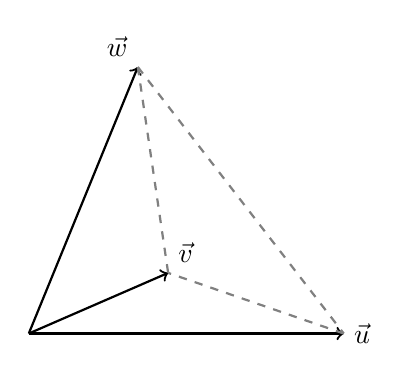
\begin{tikzpicture}
\coordinate (0) at (0,0,0);
\draw[thick, ->] (0)--(4,0,0) node[right](vecu){$\vec{u}$};
\draw[thick, ->] (0)--(1,0,-2) node[above right](vecv){$\vec{v}$};
\draw[thick, ->] (0)--(1,3,-1) node[above left](vecw){$\vec{w}$};
\draw[thick, gray, dashed] (4,0,0)--(1,0,-2);
\draw[thick, gray, dashed] (1,3,-1)--(1,0,-2);
\draw[thick, gray, dashed] (1,3,-1)--(4,0,0);
\end{tikzpicture}
\end{center}
\end{Exercise}
\begin{Answer}
It is just $\frac{1}{6}\abs{(\vec{u} \times \vec{v}) \cdot \vec{w}}$.
\end{Answer}

\begin{Exercise}
For $\vec{u} = (1,2,3)^T$, $\vec{v} = (2,1,5)^T$, $\vec{w} = (1,4,0)^T$, find
\begin{enumerate}[label=(\alph*)]
\item Area of the parallelogram formed by $\vec{u}$ and $\vec{v}$,
\item Volume of the parallelepiped formed by $\vec{u}$, $\vec{v}$ and $\vec{w}$,
\item Redo the above for $\vec{w} = (1,5,4)^T$, what does the result tell you?
\end{enumerate}
\end{Exercise}
\begin{Answer}
\begin{enumerate}[label=(\alph*)]
\item $\vec{u} \times \vec{v} =
\left|
\begin{array}{ccc}
\hat{\imath} & \hat{\jmath} & \hat{k}\\
1 & 2 & 3\\
2 & 1 & 5
\end{array}
\right|
=
7\hat{\imath} + \hat{\jmath} - 3\hat{k}$\\
Area = $\sqrt{7^2 + 1^2 + (-3)^2} = \sqrt{59}$
\item Volume is the absolute value of $|\vec{u} \times \vec{v}| \cdot \vec{w} 
= |(7\hat{\imath} + \hat{\jmath} - 3\hat{k}) \cdot (\hat{\imath} + 4\hat{\jmath})| = |(7)(1) + (1)(4) + (-3)(0)| = 11$
\item Volume = $\text{abs}\left|
\begin{array}{ccc}
1 & 2 & 3\\
2 & 1 & 5\\
1 & 5 & 4
\end{array}
\right|
= 0$. \\
So the three vectors are co-planar.
\end{enumerate}
\end{Answer}

\begin{Exercise}
Find the geometric interpretation of solutions of the following systems of linear equations.
\begin{enumerate}[label=(\alph*)]
\item 
\begin{align*}
\left\{\begin{alignedat}{2}
&x + 2y + 2z& &= 3\\
&3x - y + 3z& &= 2\\
&x - 2y - z& &= -1
\end{alignedat}\right.
\end{align*}
\item
\begin{align*}
\left\{\begin{alignedat}{2}
&2x - y - z& &= 3\\
&x + y + 2z& &= -1\\
&x + 4y + 7z& &= -6
\end{alignedat}\right.
\end{align*}
\end{enumerate}
\end{Exercise}
\begin{Answer}
\begin{enumerate}[label=(\alph*)]
\item The solution refers to the point $(1,1,0)$.
\item By Gaussian Elimination, one possible form of general solution is 
\begin{align*}
\begin{bmatrix}
x\\
y\\
z
\end{bmatrix}
=
\begin{bmatrix}
\frac{2}{3}\\
-\frac{5}{3}\\
0
\end{bmatrix}
+
t
\begin{bmatrix}
-\frac{1}{3}\\
-\frac{5}{3}\\
1
\end{bmatrix}    
\end{align*} 
Therefore, the solution space is a line parallel to 
$-\frac{1}{3}\hat{\imath} - \frac{5}{3}\hat{\jmath} + \hat{k}$ and passing through the point $(\frac{2}{3}, -\frac{5}{3}, 0)^T$.
\end{enumerate}
\end{Answer}